\documentclass[aspectratio=169,12pt]{beamer}
\usepackage{amsmath}
\usepackage{amssymb}
\usepackage[most]{tcolorbox}
\usepackage{tikz}
\usepackage{graphicx}
\usepackage[sfdefault,lf]{FiraSans}
\renewcommand{\familydefault}{\sfdefault}
\setlength{\parindent}{0pt}
\everymath{\displaystyle}

\setbeamertemplate{navigation symbols}{}
\setbeamertemplate{footline}{}
\setbeamertemplate{headline}{}

\definecolor{mmpageWhite}{HTML}{FCFBF7}
\definecolor{mmtanSoft}{HTML}{F7F5EF}
\definecolor{mmgreenDeep}{HTML}{244B2C}
\definecolor{mmgreenLeaf}{HTML}{5D8A56}
\definecolor{mmgreenSoft}{HTML}{E4EFD9}
\definecolor{mmtext}{HTML}{163221}

\setbeamercolor{background canvas}{bg=mmpageWhite}
\setbeamercolor{normal text}{fg=mmtext,bg=mmpageWhite}

\newtcolorbox{MMProblemCard}[1][]{enhanced,breakable=false,colback=white,colframe=black,boxrule=1.0pt,arc=5pt,left=3pt,right=3pt,top=2pt,bottom=2pt,before skip=0pt,after skip=0pt,height=0.26\textheight,valign=top,#1}
\newcommand{\KoruIcon}{\raisebox{-0.2em}{
\includegraphics[height=1.05em]{../../SITE/header-logo.png}}}
\newcommand{\HoeIcon}{\raisebox{-0.2em}{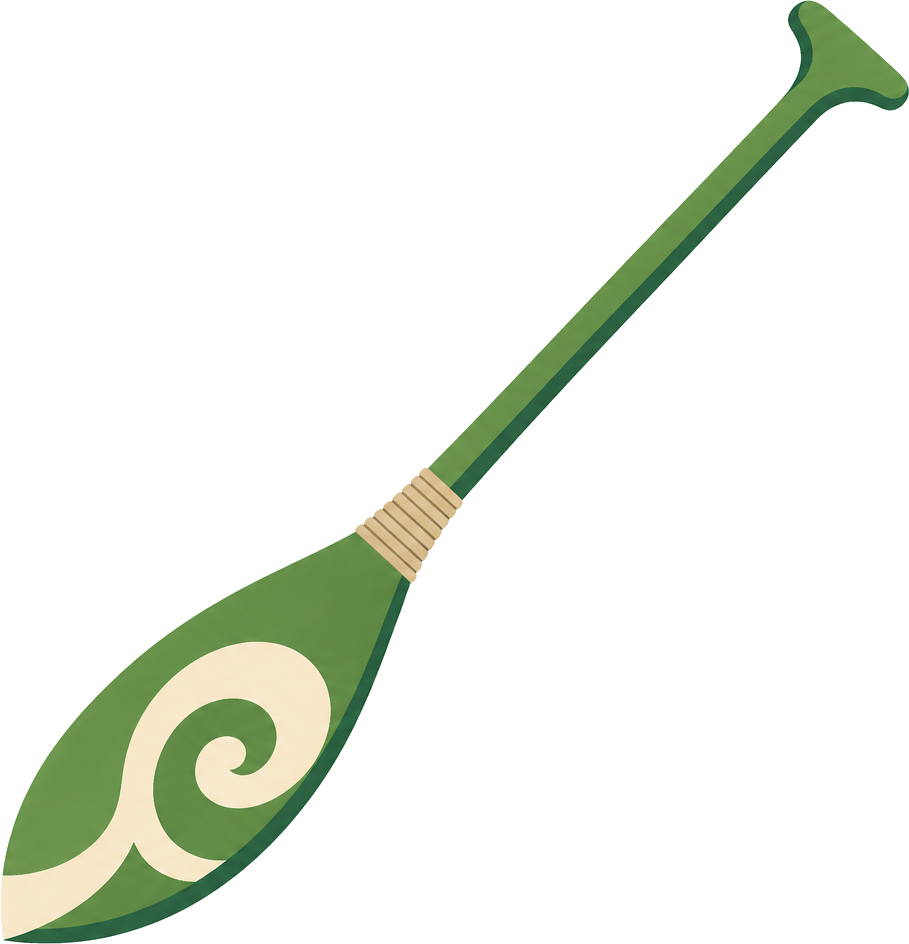
\includegraphics[height=1.05em]{../../SITE/hoe.png}}}
\newcommand{\ScaffoldIcons}[1]{\ifcase#1\or \HoeIcon\or \HoeIcon\hspace{0.22em}\KoruIcon\or \KoruIcon\hspace{0.22em}\KoruIcon\hspace{0.22em}\KoruIcon\fi}
\newcommand{\WorksheetTitle}[2]{%
  {\colorbox{mmtanSoft}{\parbox[c][2.0em][c]{0.975\linewidth}{%
    \hspace{0.25em}{\Large\bfseries\textcolor{mmgreenDeep}{#1}\hfill\ScaffoldIcons{#2}}}}
  \par\vspace{0.08em}{\color{mmgreenLeaf}\rule{\linewidth}{2.0pt}}\par\vspace{0.04em}}
}
\newcommand{\MMProblem}[2]{\begin{MMProblemCard}\raggedright\small\textbf{#1.} #2\par\end{MMProblemCard}}

\setbeamertemplate{background}{
 \begin{tikzpicture}[remember picture,overlay]
 \draw[black,line width=1.5pt,rounded corners=10pt]
 ([xshift=0.45cm,yshift=-0.45cm]current page.north west)
 rectangle
 ([xshift=-0.45cm,yshift=0.45cm]current page.south east);
 \end{tikzpicture}
}

% Default worksheet generation rules:
% use notes-style beamer pages
% use bordered cards for individual problems
% target 9 problems per frame in a 3x3 grid
% target 3 frames per scaffold by default where content allows

\begin{document}\begin{frame}[t]
\WorksheetTitle{Start Tasks}
\vspace{-0.18em}
\begin{columns}[T,onlytextwidth]
\begin{column}{0.32\textwidth}\MMProblem{1}{Two straight lines cross. One angle is \mbox{$68^\circ$}. The vertically opposite angle is \mbox{$x$}. Find \mbox{$x$}.}\end{column}
\begin{column}{0.32\textwidth}\MMProblem{2}{Two straight lines cross. One angle is \mbox{$95^\circ$}. The vertically opposite angle is \mbox{$y$}. Find \mbox{$y$}.}\end{column}
\begin{column}{0.32\textwidth}\MMProblem{3}{Two straight lines cross. One angle is \mbox{$53^\circ$}. The vertically opposite angle is \mbox{$a$}. Find \mbox{$a$}.}\end{column}
\end{columns}
\vspace{0.45em}
\begin{columns}[T,onlytextwidth]
\begin{column}{0.32\textwidth}\MMProblem{4}{Two straight lines cross. One angle is \mbox{$41^\circ$}. The vertically opposite angle is \mbox{$b$}. Find \mbox{$b$}.}\end{column}
\begin{column}{0.32\textwidth}\MMProblem{5}{Two straight lines cross. One angle is \mbox{$106^\circ$}. The vertically opposite angle is \mbox{$c$}. Find \mbox{$c$}.}\end{column}
\begin{column}{0.32\textwidth}\MMProblem{6}{Two straight lines cross. One angle is \mbox{$118^\circ$}. The vertically opposite angle is \mbox{$d$}. Find \mbox{$d$}.}\end{column}
\end{columns}
\vspace{0.45em}
\begin{columns}[T,onlytextwidth]
\begin{column}{0.32\textwidth}\MMProblem{7}{Write the rule that links vertically opposite angles.}\end{column}
\begin{column}{0.32\textwidth}\MMProblem{8}{One angle is \mbox{$33^\circ$}. What is the vertically opposite angle?}\end{column}
\begin{column}{0.32\textwidth}\MMProblem{9}{One angle is \mbox{$146^\circ$}. What is the vertically opposite angle?}\end{column}
\end{columns}
\end{frame}
\begin{frame}[t]
\WorksheetTitle{Start Tasks}
\vspace{-0.18em}
\begin{columns}[T,onlytextwidth]
\begin{column}{0.32\textwidth}\MMProblem{1}{Two straight lines cross. One angle is \mbox{$142^\circ$}. The vertically opposite angle is \mbox{$m$}. Find \mbox{$m$}.}\end{column}
\begin{column}{0.32\textwidth}\MMProblem{2}{Two straight lines cross. One angle is \mbox{$84^\circ$}. The vertically opposite angle is \mbox{$n$}. Find \mbox{$n$}.}\end{column}
\begin{column}{0.32\textwidth}\MMProblem{3}{A student says vertically opposite angles add to \mbox{$180^\circ$}. Correct the statement.}\end{column}
\end{columns}
\vspace{0.45em}
\begin{columns}[T,onlytextwidth]
\begin{column}{0.32\textwidth}\MMProblem{4}{Two straight lines cross. One angle is \mbox{$125^\circ$}. The vertically opposite angle is \mbox{$p$}. Find \mbox{$p$}.}\end{column}
\begin{column}{0.32\textwidth}\MMProblem{5}{Explain in one short sentence how you spot vertically opposite angles in a crossing-lines diagram.}\end{column}
\begin{column}{0.32\textwidth}\MMProblem{6}{}\end{column}
\end{columns}
\vspace{0.45em}
\begin{columns}[T,onlytextwidth]
\begin{column}{0.32\textwidth}\MMProblem{7}{}\end{column}
\begin{column}{0.32\textwidth}\MMProblem{8}{}\end{column}
\begin{column}{0.32\textwidth}\MMProblem{9}{}\end{column}
\end{columns}
\end{frame}
\end{document}
